\section{Evaluation} \label{sec:evaluation}


\subsection{Performance}



\subsubsection{Unbalanced tree search in memory}


%Using 6 cores per node gave
%Grappa up to a 20\% benefit at each data point, but Grappa could not run
%well beyond 90 machines with this core configuration because of the
%current network aggregator designa.

We ran UTS-mem on Grappa and the XMT with a binomial and two geometric
100M-vertex trees (T3L,T1L,T2L), a geometric 1.6B-vertex tree (T1XL),
and a geometric 4.2B-vertex tree (T1XXL). Both systems do relatively
poorly on the binomial tree because it is very deep and a traversal
produces too little parallelism. Figure~\ref{fig:uts_compare} shows
the performance in terms of number of vertices visited per second versus
number of compute nodes. The Grappa results shown are for 6 cores per
node and the best parameter values from a search over runtime and
application parameters.



%% UTS: performance comparison
\begin{figure}[ht]
    \begin{center}
      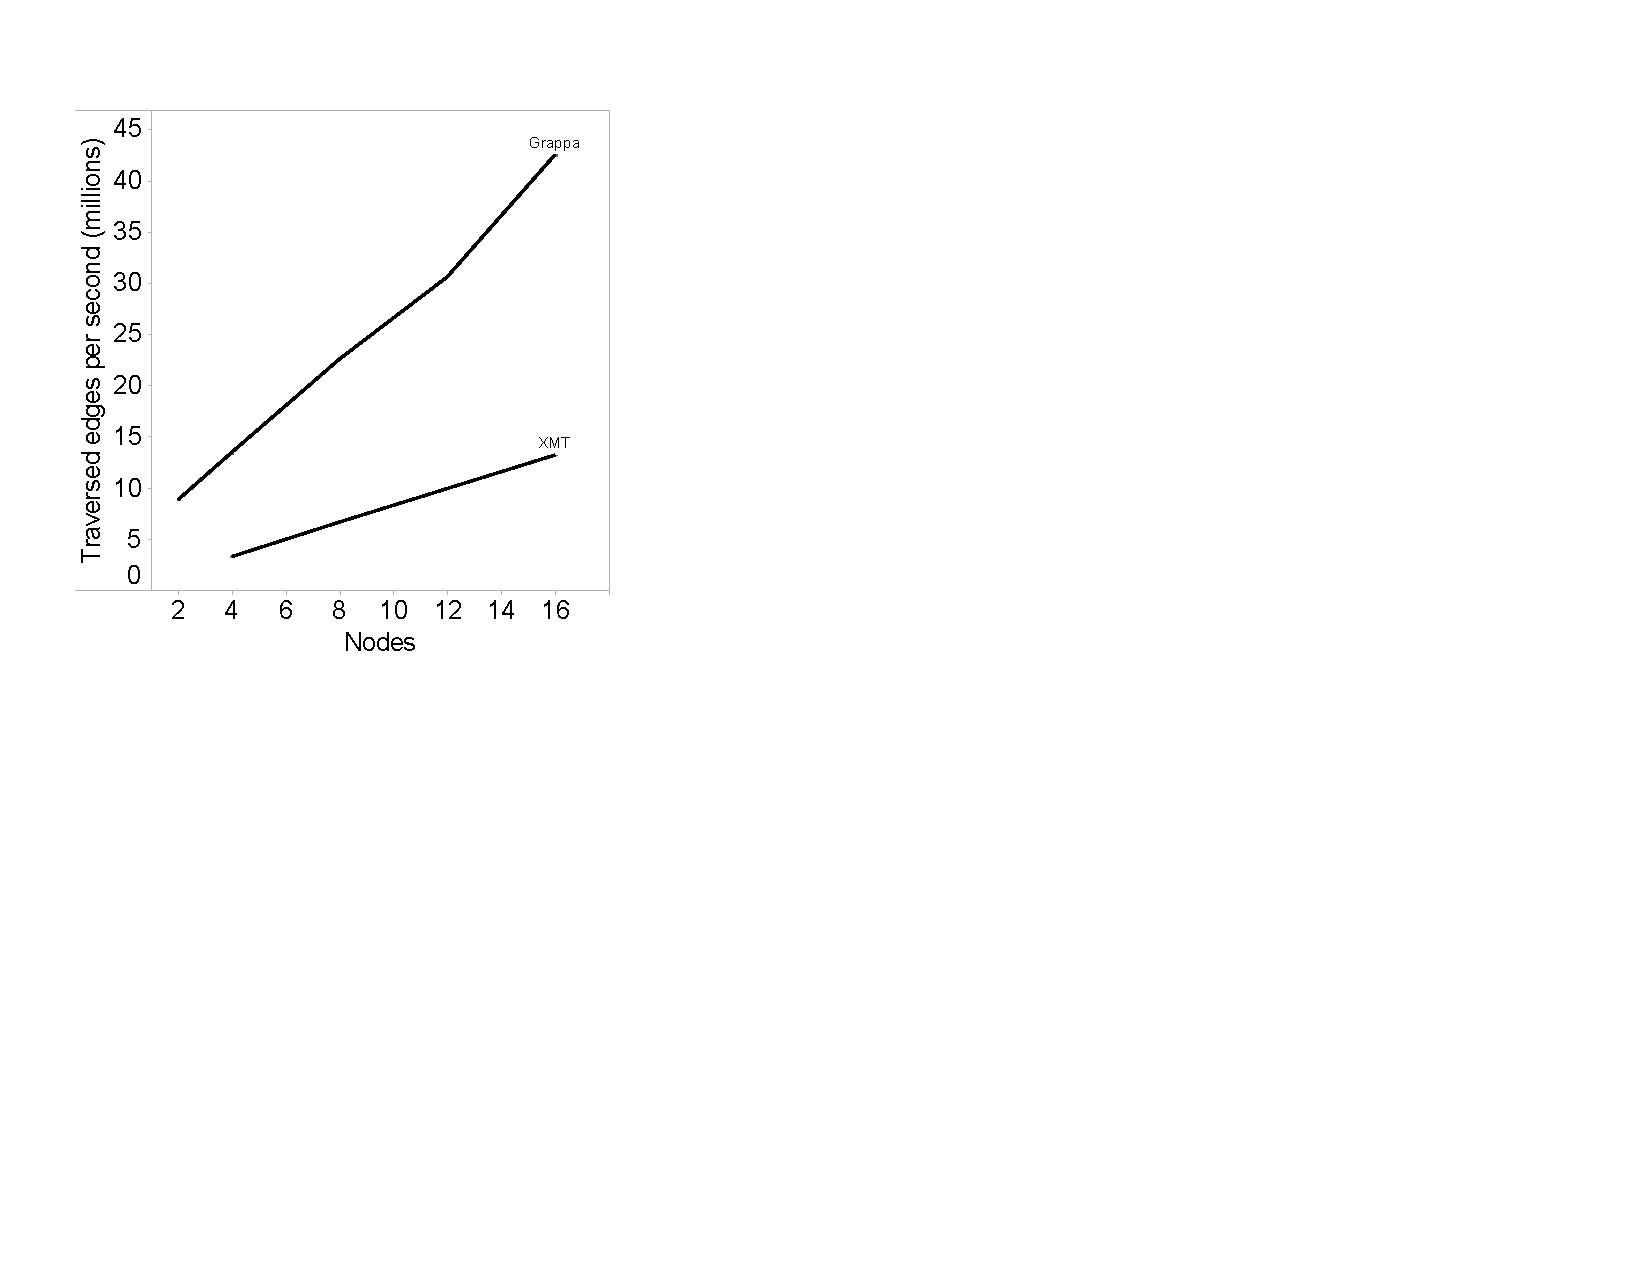
\includegraphics[width=0.5\textwidth]{figs/uts_performance.pdf}
    \end{center}
    \caption{Performance of in-memory unbalanced tree search.}
    \label{fig:uts_compare}
\end{figure}


\TODO{ we still win with th=1 }

\subsubsection{BFS}

\begin{figure}[tH]
\begin{center}
  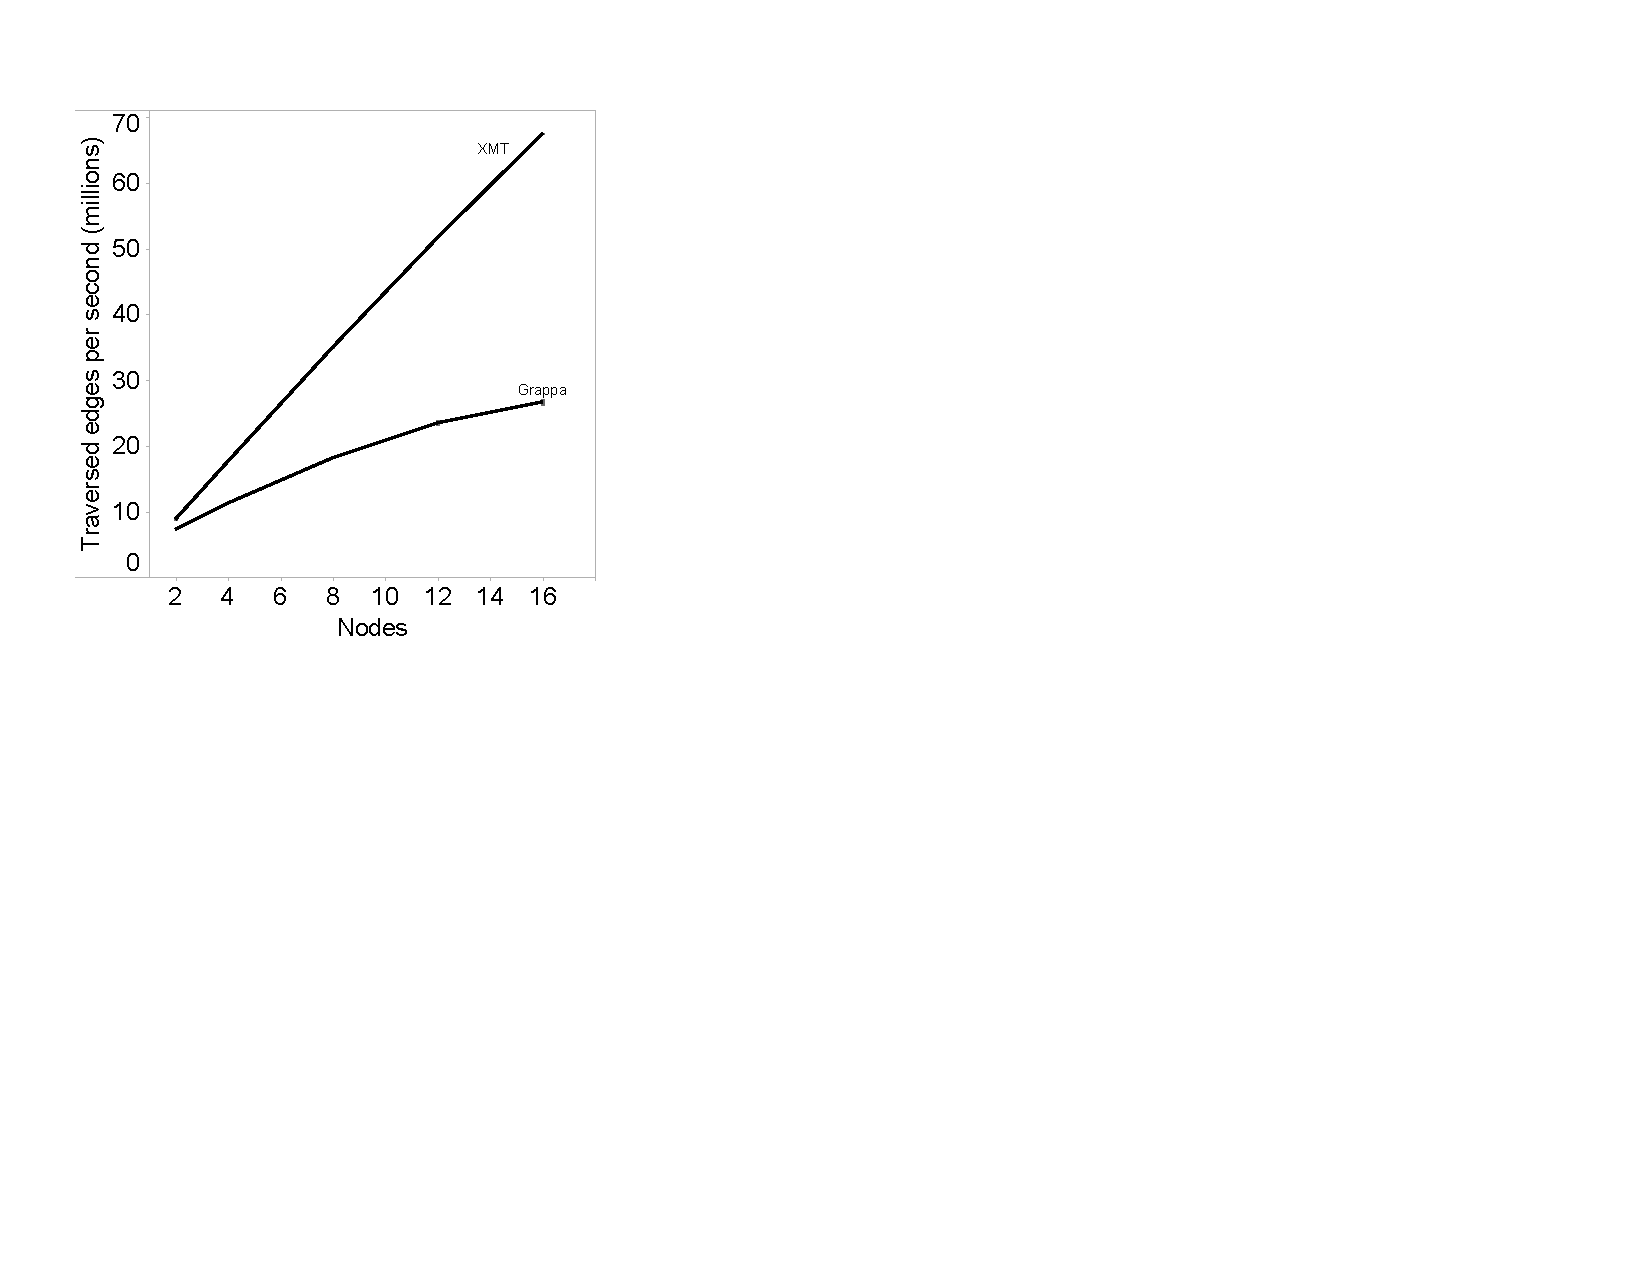
\includegraphics[width=0.95\columnwidth]{figs/bfs_performance}
\begin{minipage}{0.95\columnwidth}
  \caption{\label{fig:bfs-performance} BFS performance}
\end{minipage}
\vspace{-3ex}
\end{center}
\end{figure}

Figure~\ref{fig:bfs-performance} shows Grappa's performance on BFS
compared to that of the XMT.\footnote{The performance dip at 112 nodes is not an anomaly; it is highly repeatable.  Despite extensive investigation on our part, we can find no reasonable explanation for it.} There are
two things to observe. First, At 128 XMT processors/cluster nodes,
the XMT is  4.17 times faster than Grappa. This is due to the
XMT's faster network: the XMT is able to issue 100 million network
requests per second per node; at the 128 nodes datapoint, Grappa is
aggregating 25 million network requests per second, or 4 times slower.
\checkme{Second, Grappa is scaling...}

\subsubsection{Centrality}

\begin{figure}[tH]
\begin{center}
  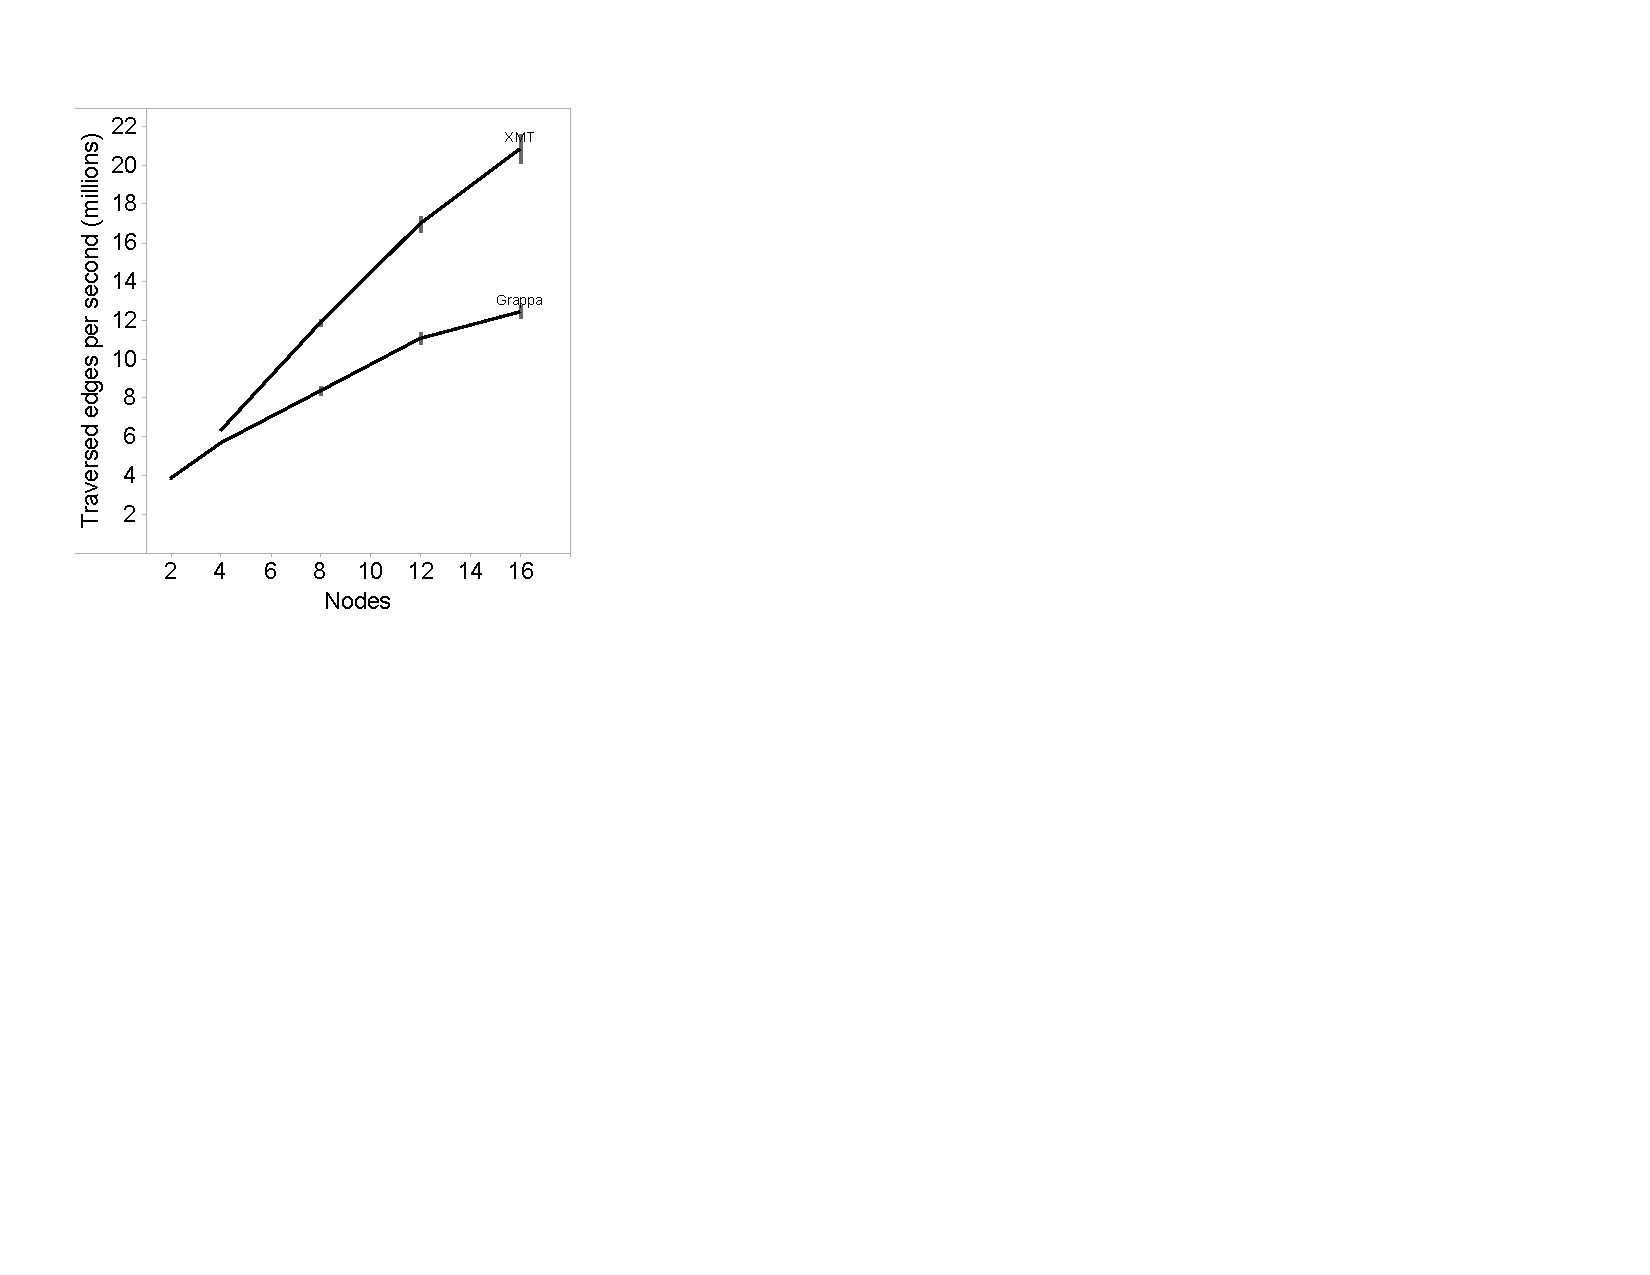
\includegraphics[width=0.95\columnwidth]{figs/centrality_performance}
\begin{minipage}{0.95\columnwidth}
  \caption{\label{fig:centrality-performance} Centrality performance}
\end{minipage}
\vspace{-3ex}
\end{center}
\end{figure}

Figure~\ref{fig:centrality-performance} shows Grappa's performance on
Betweenness Centrality compared to that of the XMT. At 128 XMT
processors/cluster nodes, the XMT is 1.75 times faster than Grappa.
\TODO{Add more here...}

\subsection{Network aggregation performance}


\begin{figure}[htbH]
\begin{center}
  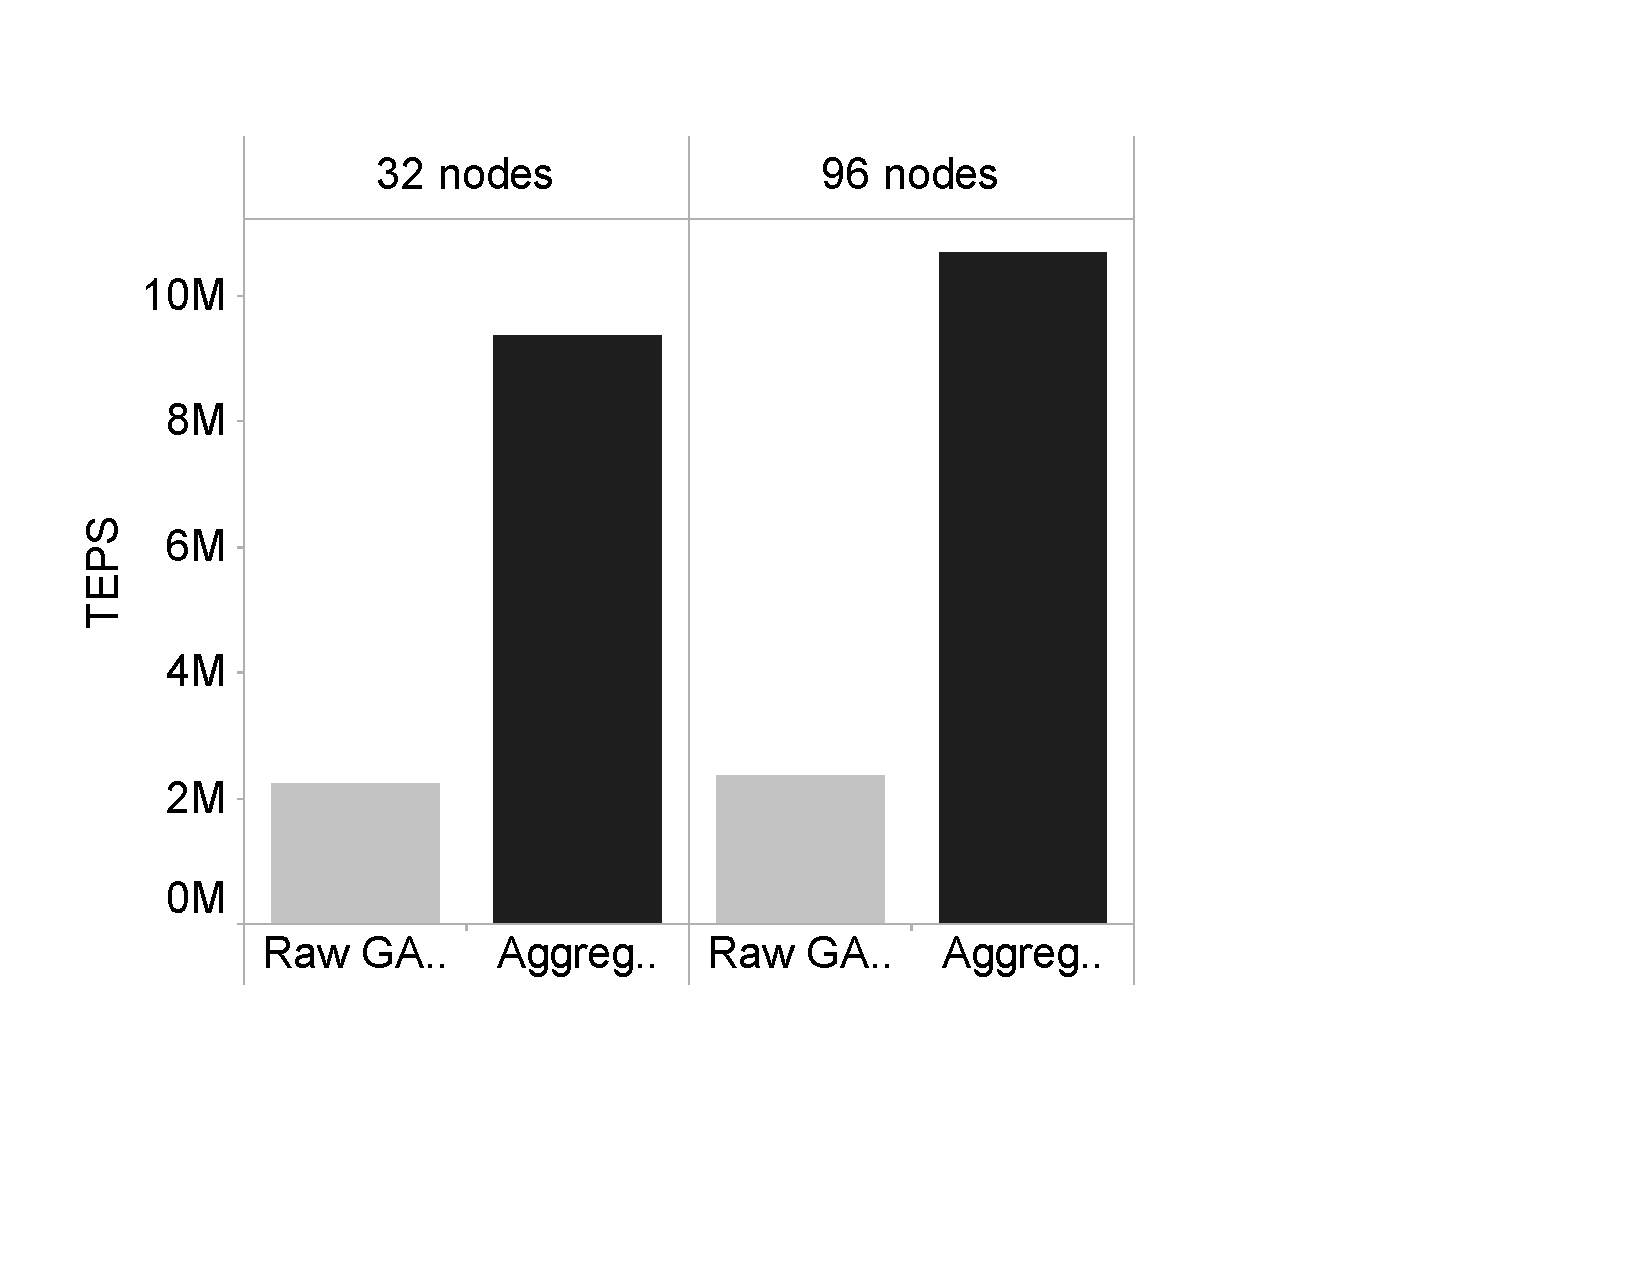
\includegraphics[width=0.95\columnwidth]{figs/bfs_aggregator_value}
\begin{minipage}{0.95\columnwidth}
  \caption{\label{fig:bfs-aggregator} BFS performance with and without aggregator enabled \TODO{This graph sucks; rerun on actual data point and include in performance comparison}}
\end{minipage}
\vspace{-3ex}
\end{center}
\end{figure}




\begin{figure}[htb]
\begin{center}
  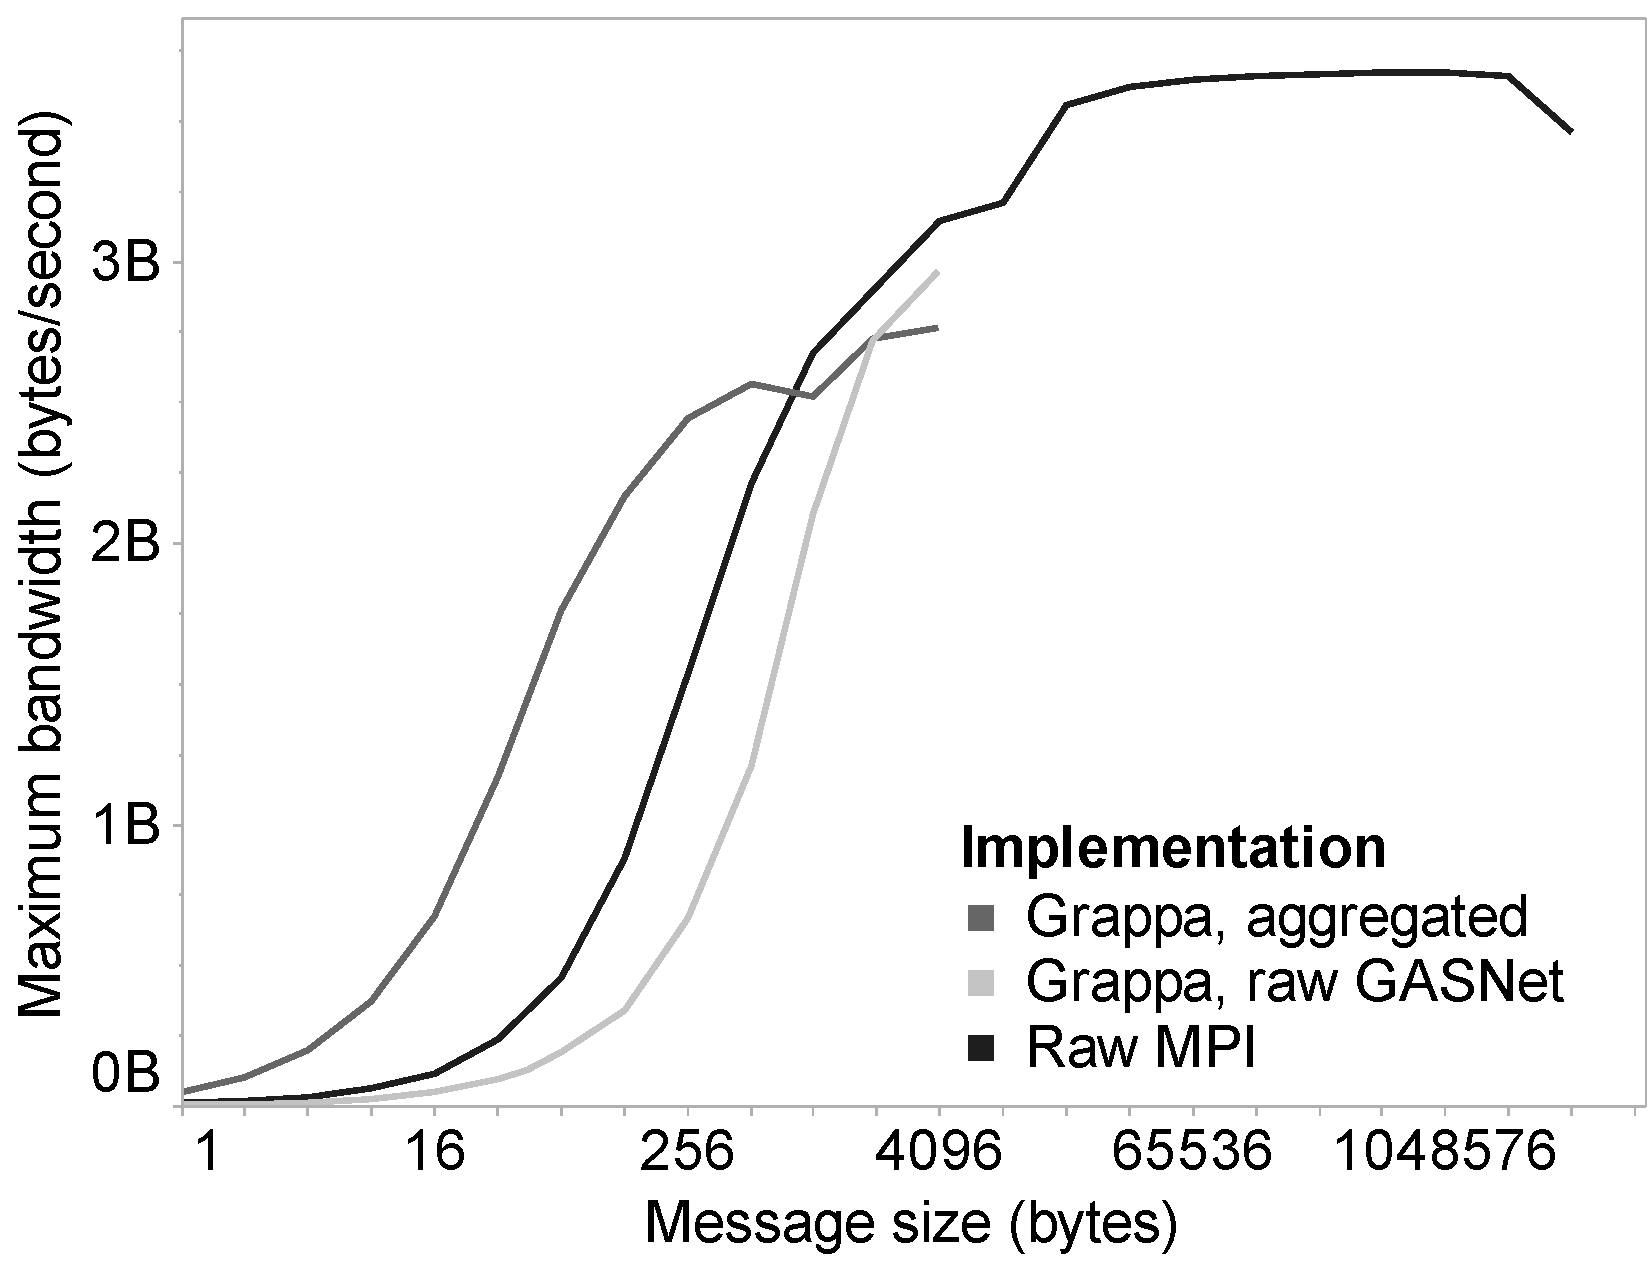
\includegraphics[width=0.95\columnwidth]{figs/aggregator_ping}
\begin{minipage}{0.95\columnwidth}
  \caption{\label{fig:aggregator-ping} Bandwidth versus message size
    unidirectional ping test for Grappa with aggregation, Grappa with
    raw GASNet messages, and MPI. Aggregation provides an 11x
    bandwidth benefit at our common operating point.}
\end{minipage}
\vspace{-3ex}
\end{center}
\end{figure}

To evaluate the benefits of network aggregation, we ran two experiments.
First, we ran a simple unidirectional ping test to see the maximum
benefit the aggregator can provide in terms of improved network
efficiency. Second, we ran BFS with the aggregator disabled in order to
measure its benefit on an application.

To implement the ping test, we wrote a simple Grappa application where
the cores of one node send messages as fast as possible to the cores
of another node. We vary the size of the payload up the maximum
payload size supported by the aggregator (nearly 4KB). Each core has a
single task sending to a single destination, so this is a best case
scenario for the aggregator. To see the benefit of the aggregator, we
added a bypass that lets us send messages directly through GASNet. We
also compare against the OSU \texttt{osu\_mbw\_mr} benchmark
\TODO{cite?}  compiled against OpenMPI 1.5.3 \TODO{cite?}; this
benchmark has the same pattern of communication but doesn't have the
overhead of Grappa's context switching.

The results are shown in Figure~\ref{fig:aggregator-ping}. There are
two key observations.

First, small message performance against the existing libraries is, as expected, poor. The MPI application test shows us that peak per node
bandwidth supported by our infiniband card is 3.4GB/s. This is
achievable only with large messages; we must send 16KB packets to get
within 5 percent of peak bandwidth. But in our benchmarks, we saw
average message between 32 and 64 bytes. At 32 bytes, the MPI test is
using less than 7 percent of its peak bandwidth. Grappa sending
messages directly through GASNet uses less than 3 percent of the peak
bandwidth.

Second, aggregation has the potential to improve this situation by an
order of magnitude. With aggregation, Grappa is able to send 32-byte
messages over 12 times faster than using GASNet directly. This is a
more respectable 32 percent of peak bandwidth. Due to expedient design
decisions, Grappa's aggregator limits its aggregation to 4KB; this
limits its peak achievable bandwidth to 75 percent of the actual
peak.

But this comparison is the best possible case for the aggregator. In
order to verify that the aggregator still has value on actual
applications at scale, we ran a small (scale 20 \TODO{run larger}) BFS
with the aggregator disabled, with both 32 and 96
nodes. Figure~\ref{fig:bfs-aggregator} shows the results. With 96
nodes, the aggregator improves our application performance by 4 times.

\subsection{Sensitivity}

\paragraph{Aggregator timeout}

\begin{figure}[htb]
\begin{center}
  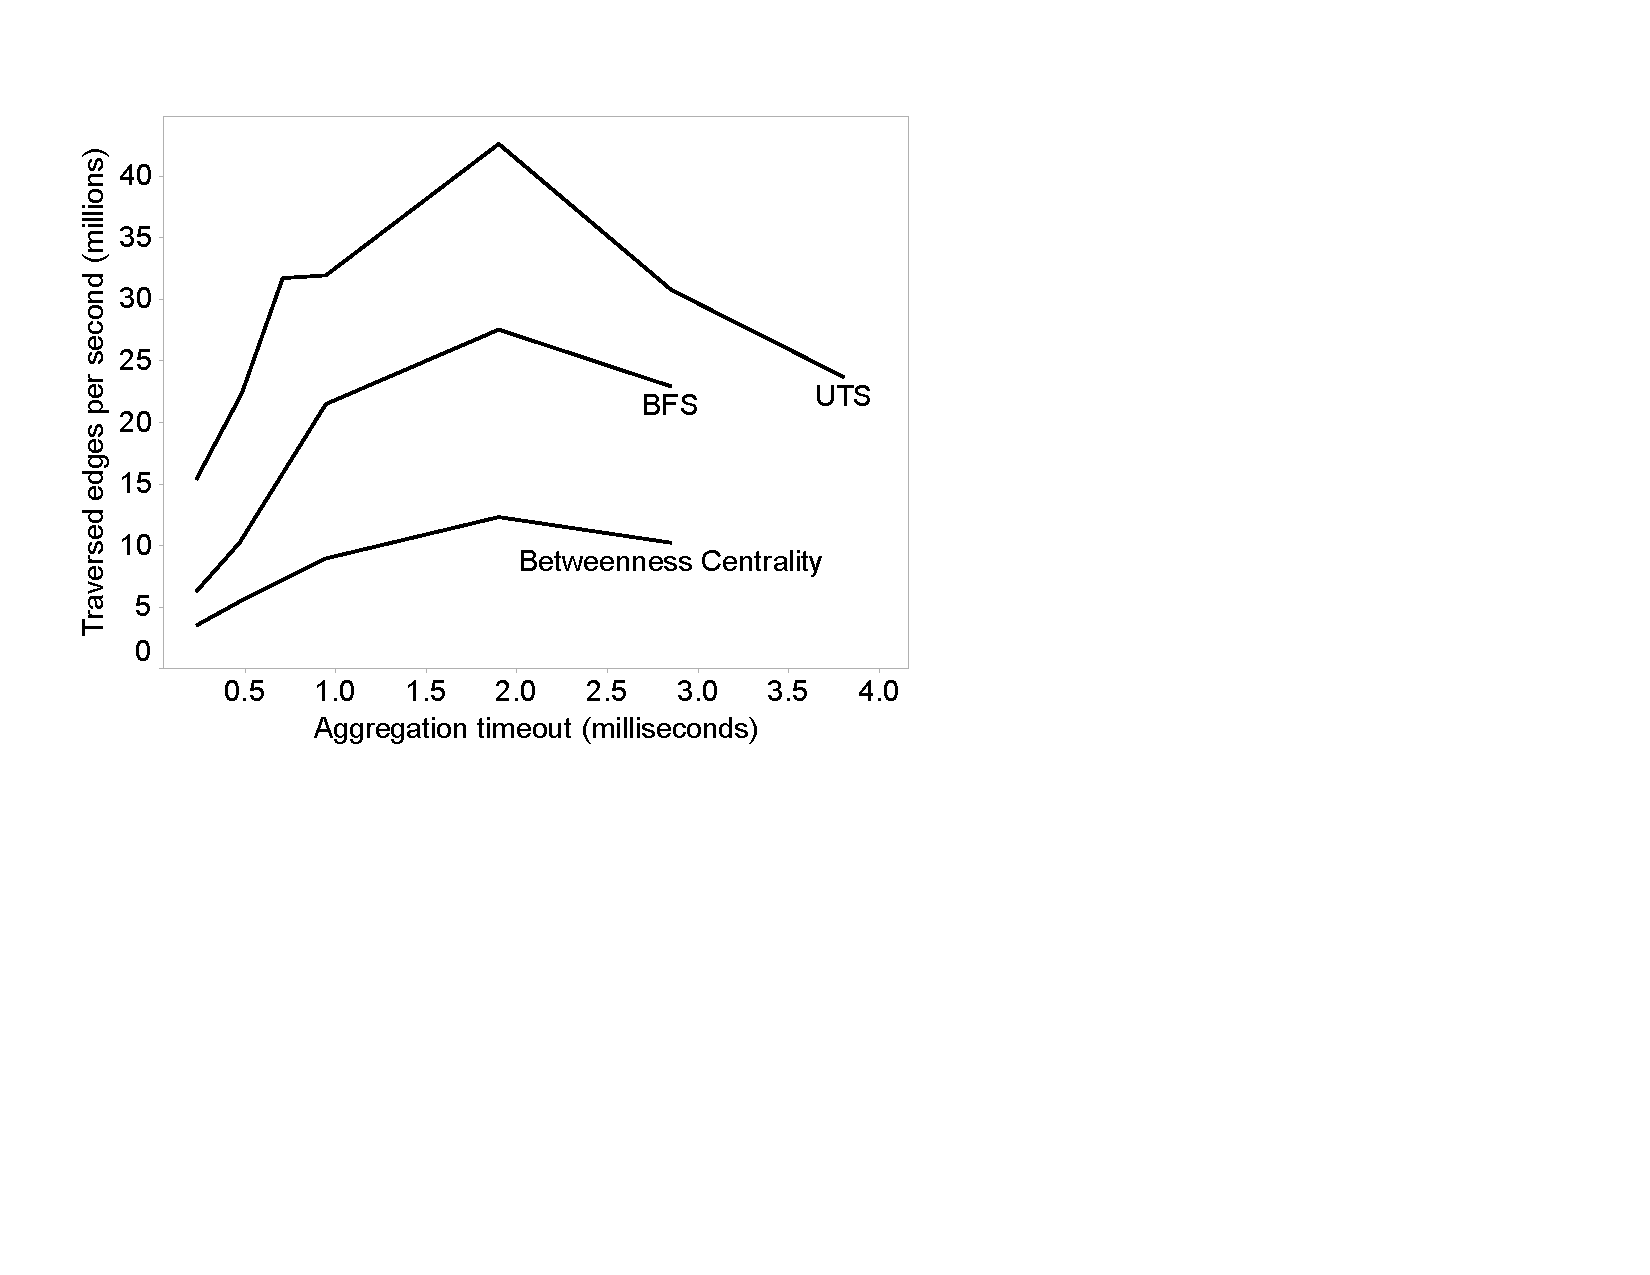
\includegraphics[width=0.95\columnwidth]{figs/flushticks_sweep}
\begin{minipage}{0.95\columnwidth}
  \caption{\label{fig:bfs-sweep-flushticks} Sensitivity to aggregation delay}
\end{minipage}
\vspace{-3ex}
\end{center}
\end{figure}


One of the key parameters of the aggregator is the message
timeout. All messages that are queued must eventually be sent in order
to ensure progress. In the best case, we are able to aggregate enough
messages to fill an aggregation buffer and cause it to be sent, but as
we scale up, the average rate of messages heading to a common
destination decreases, and this gets harder. To bound the problem, the
aggregator includes a timeout. Any packet waiting this long must be sent.

Figure~\ref{fig:bfs-sweep-flushticks} shows a sweep of this parameter
for 32-node and 96-node BFS runs. The optimal timeout value varies
with the size of the job. In the 32-node job, performance peaks with a
2 ms timeout; with the 96-node job, performance peaks with a 14 ms
timeout.

\begin{figure}[htb]
\begin{center}
  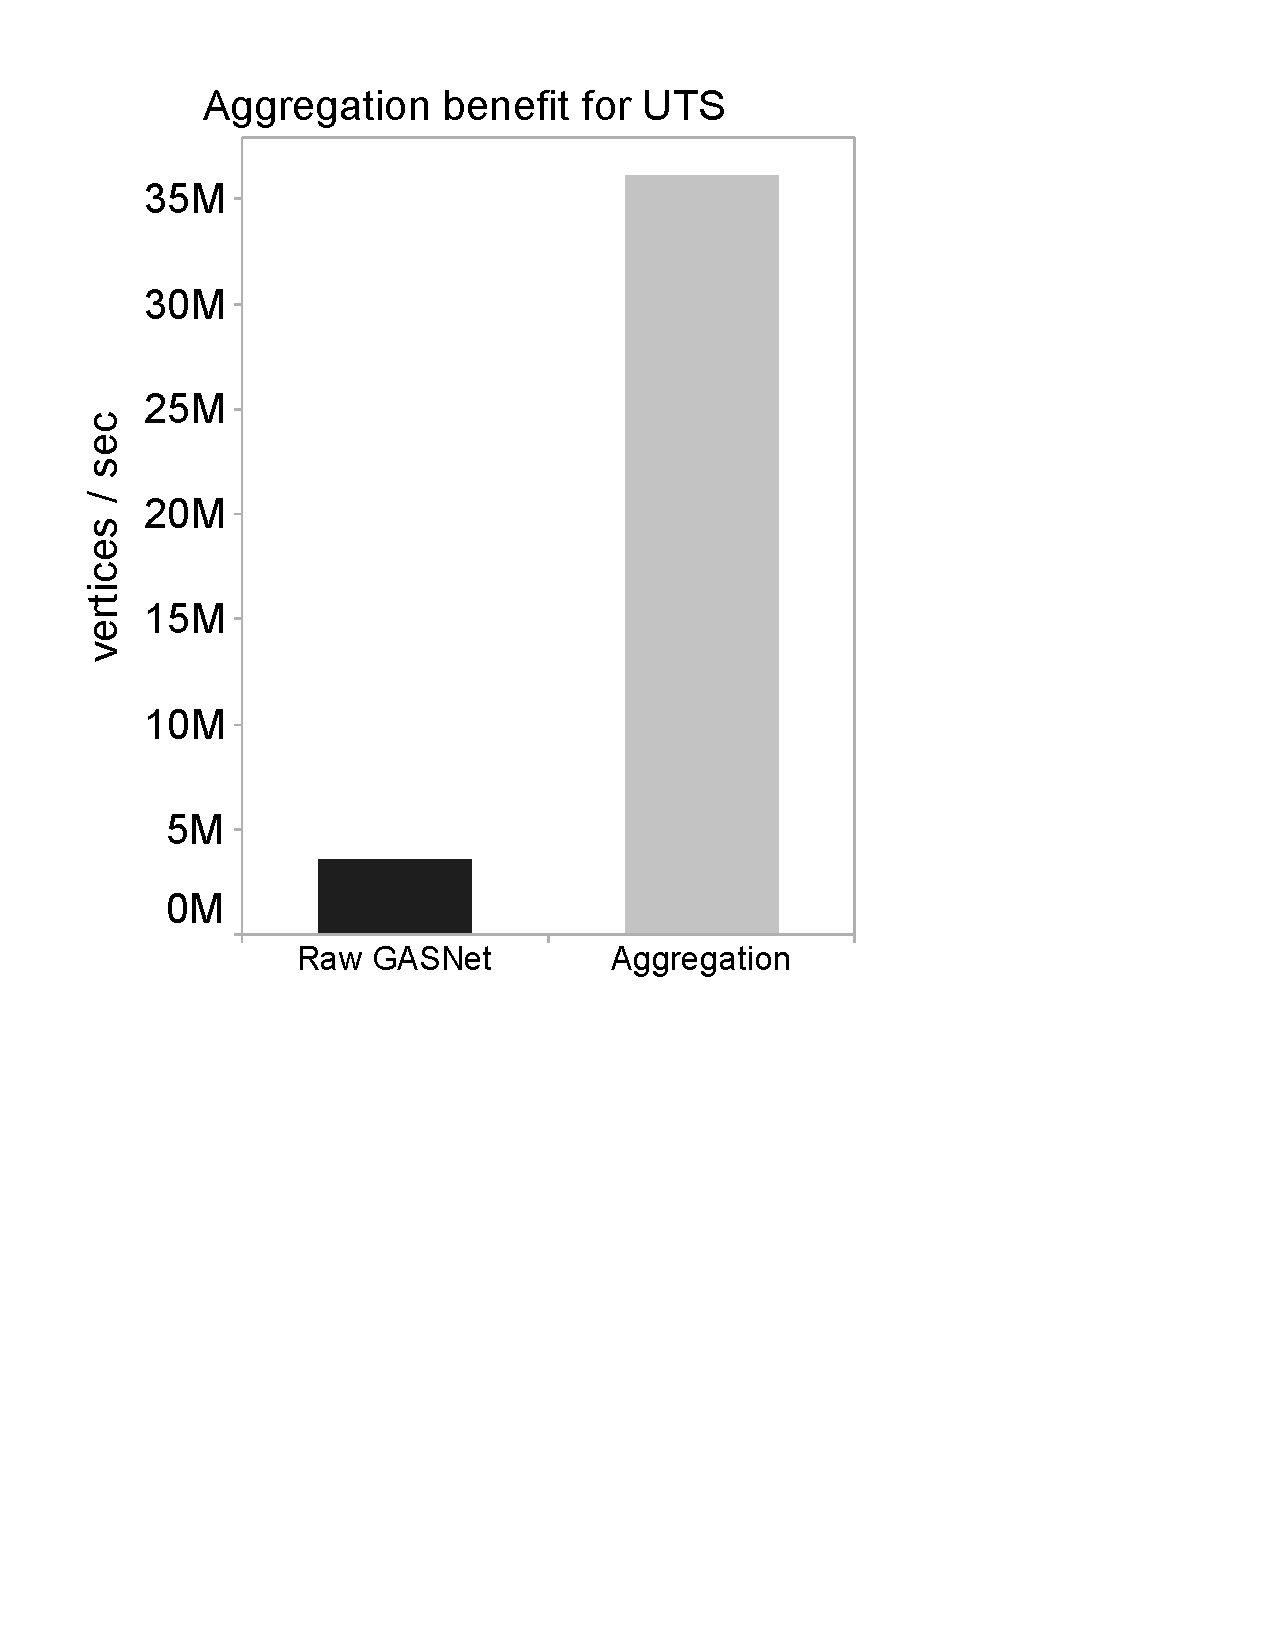
\includegraphics[width=0.95\columnwidth]{figs/no_aggregation_uts.pdf}
\begin{minipage}{0.95\columnwidth}
  \caption{\label{fig:no-aggregation-uts} Performance of UTS on 16
      nodes with and without Grappa's aggregation.}
\end{minipage}
\vspace{-3ex}
\end{center}
\end{figure}

\paragraph{Number of active tasks}


\begin{figure}[htb]
\begin{center}
  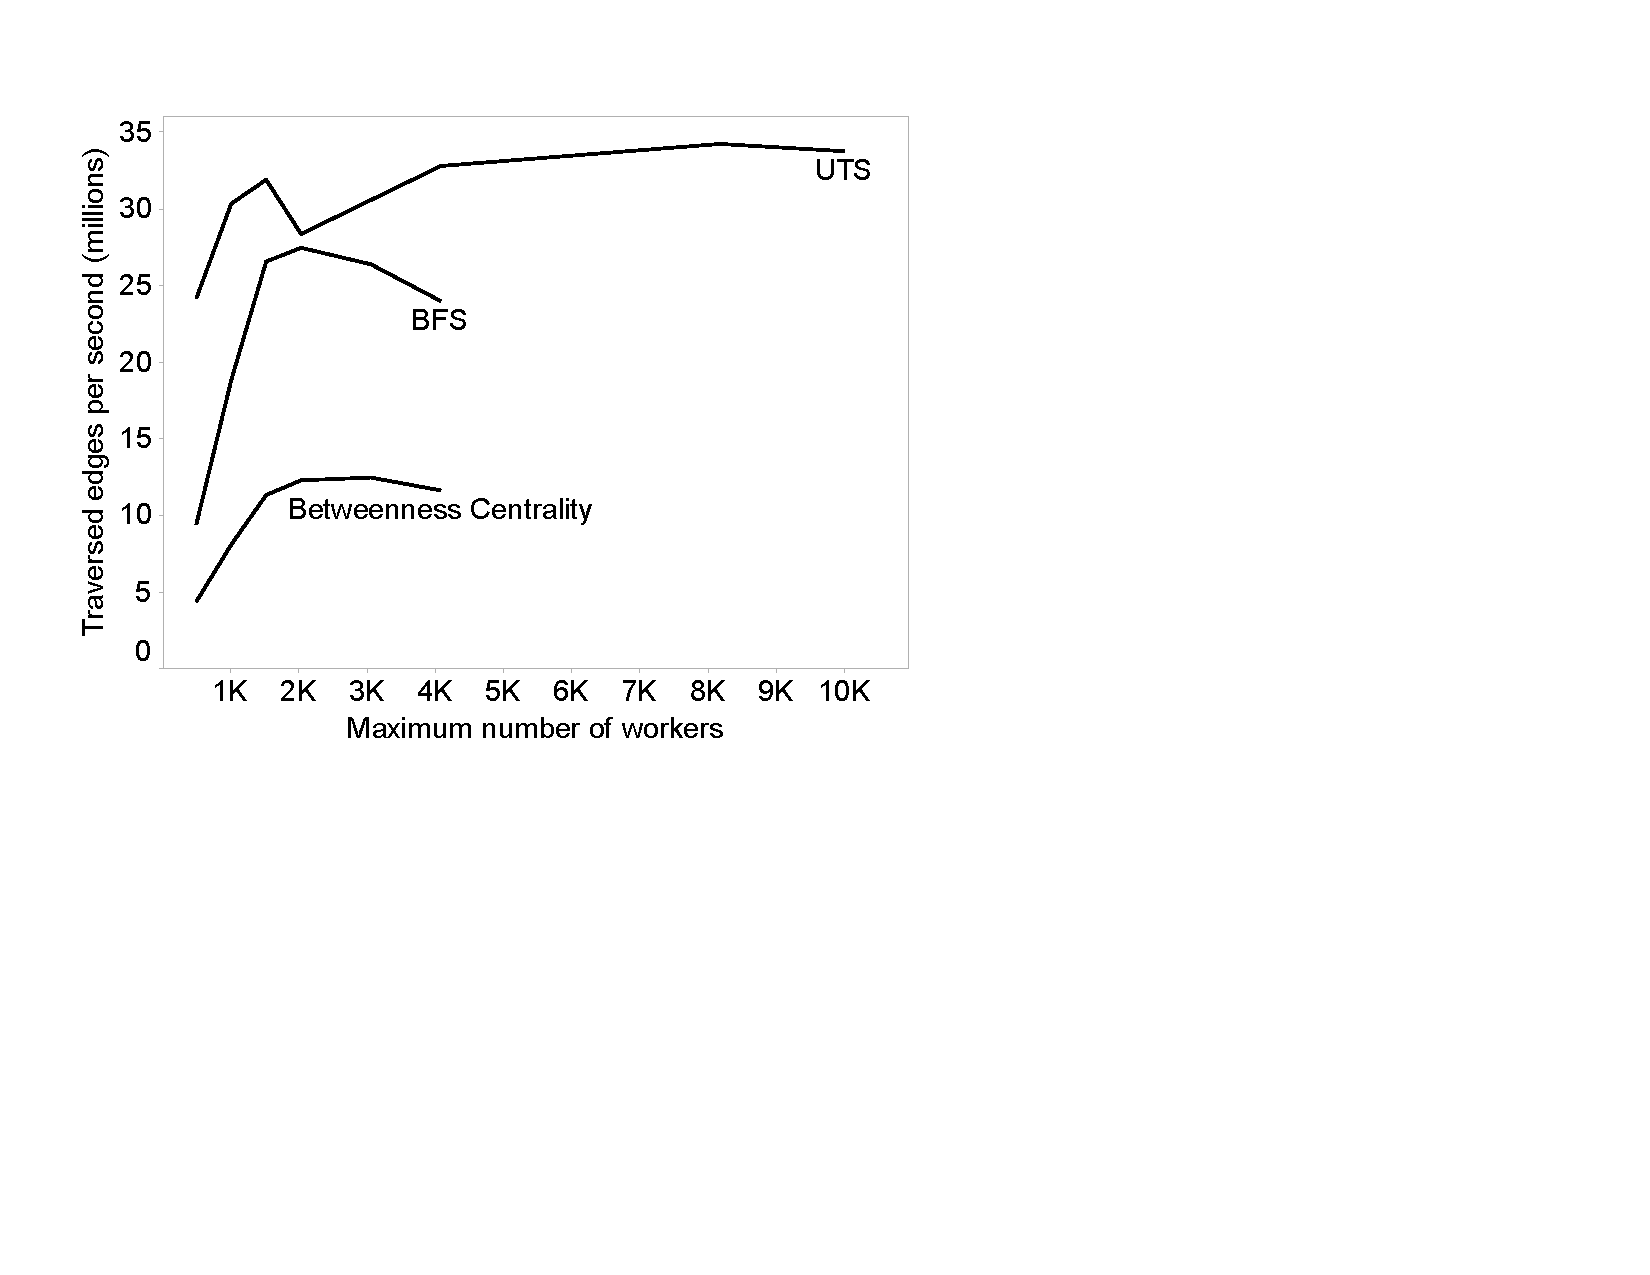
\includegraphics[width=0.95\columnwidth]{figs/worker_sweep}
\begin{minipage}{0.95\columnwidth} 
  \caption{\label{fig:bfs-sweep-workers} Sensitivity to maximum active tasks}
\end{minipage}
\vspace{-3ex}
\end{center}
\end{figure}

When a task issues a request that requires a response, it blocks to
allow other tasks to utilize its core. These tasks may also block. To
support the many milleseconds of latency aggregation adds, we need to
support many thousands of blocked tasks. One of the key parameters of
the runtime is the number of blocked tasks allowed; we need enough to
cover the network and aggregation latency, but too many running tasks
can add extra latency as they all must be multiplexed onto the same core.

Figure~\ref{fig:bfs-sweep-workers} shows a sweep of the maximum number
of active tasks per core, holding all other parameters
constant. Again, the optimal value varies with the size of the
run. For 32 nodes, a maximum of 3072 active tasks per core gives the
best result; for 96 nodes, 16000 tasks is best. 

\subsubsection{Work stealing parameters}

\paragraph{Chunk size}

It is important to steal multiple tasks at a time to both amortize the
cost of stealing over the network and to spread out work quickly in a
large system. Figure~\ref{fig:ut_chunksize} shows performance and
stealing statistics for UTS on \checkme{30} nodes as we increase the stealing chunk size. Recall
that a thief will take a number of tasks equal to the minimum of half
the available work or the chunk size; steals fail only when the victim
has fewer than 2 available tasks. As the scheduler is allowed to
steal more work beyond 1 task, we see that performance increases up to 6x. This
shows that the heuristic of stealing the oldest task from victims is
insufficient alone when a tree-structured computation is imbalanced,
as observed in \cite{UTS}. By observing sampled state in the execution
trace, we find that a chunk size as low as 1 allows stealing to
spread the load evenly across the cluster but cores spend much time
underutilized as multiple workers wait for steal replies that
utlimately return little new work.

Performance plateaus before maximum steal amount is limited by the
size of the victim's task queue. This indicates that artificially limiting steals
to \checkme{128} tasks does not limit performance. Although a lower
chunk size limits how quickly work spreads, for sufficient chunk size,
the heuristic of stealing the oldest tasks from victims in tree-based computations allows for
stolen work to expand quickly.


%% UTS: chunk size
\begin{figure}[ht]
    \begin{center}
      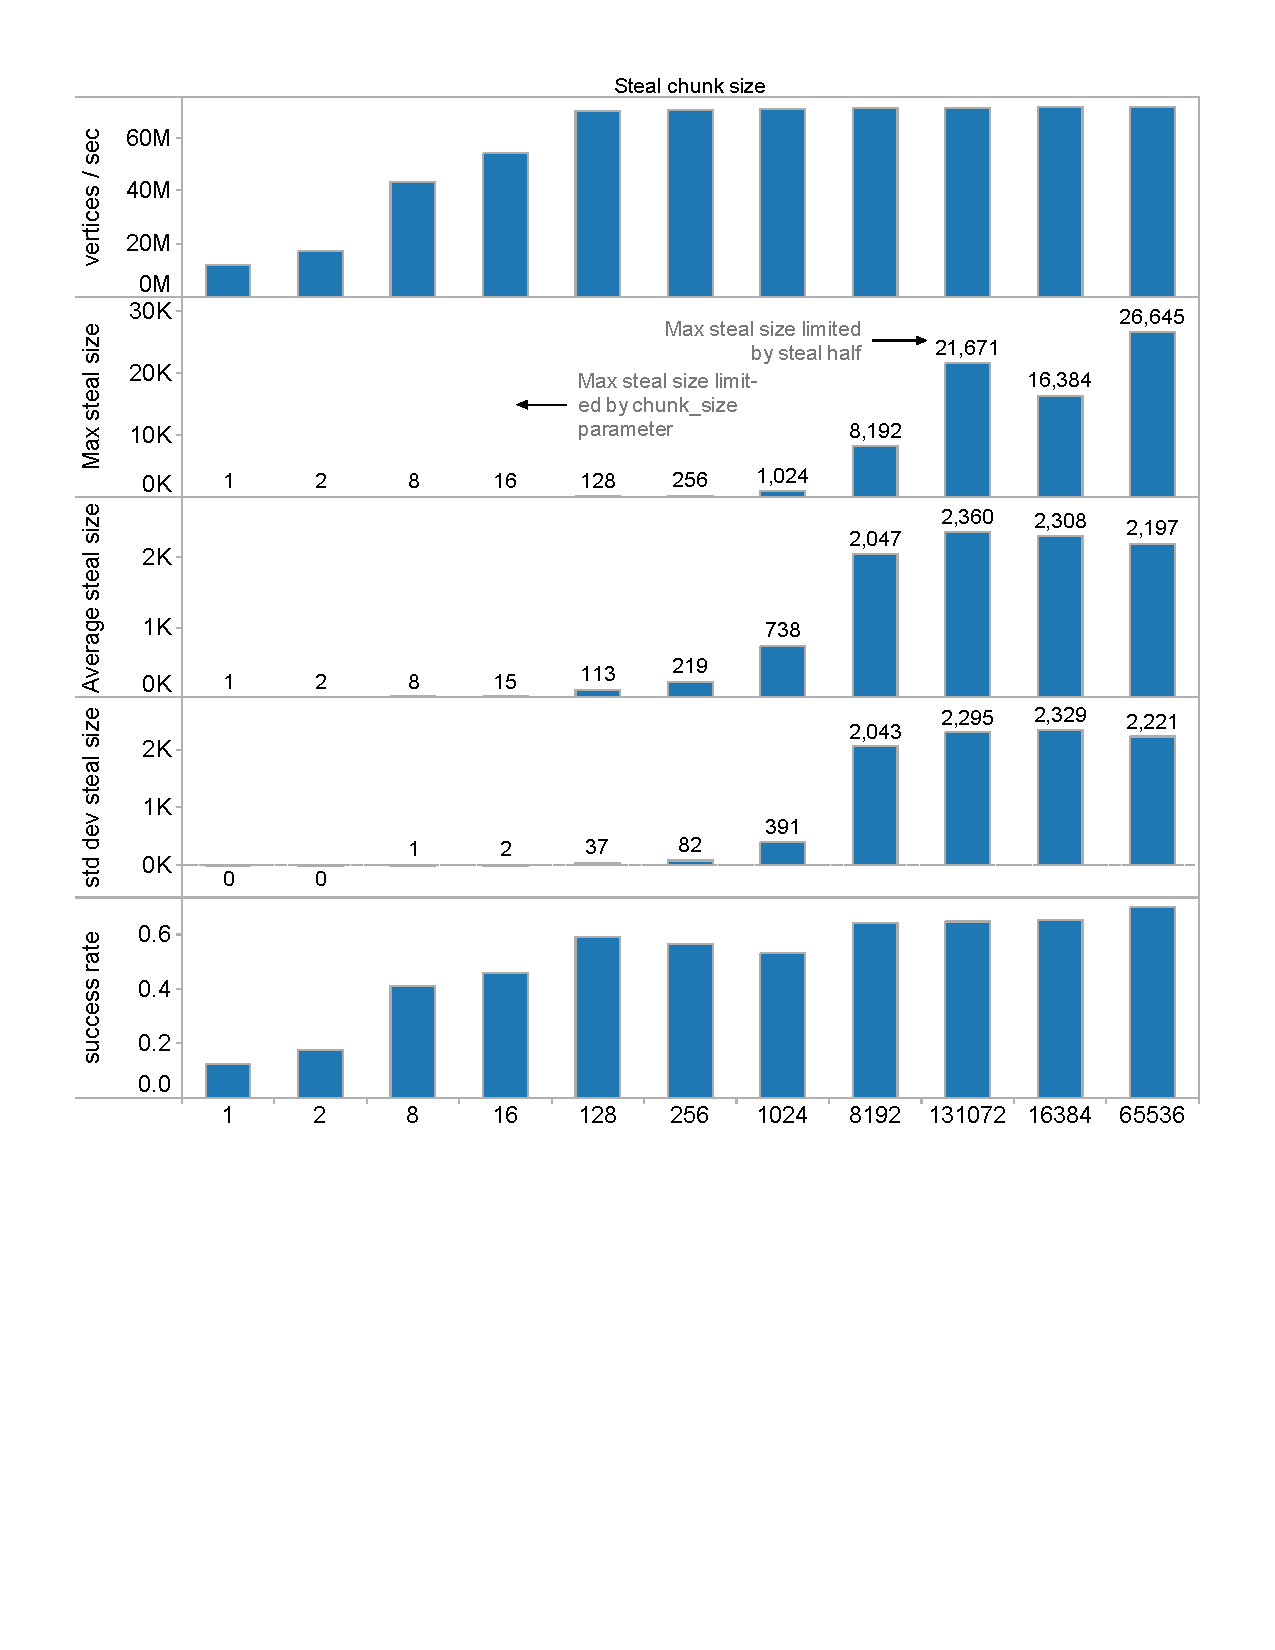
\includegraphics[width=0.5\textwidth]{figs/uts_chunksize.pdf}
    \end{center}
    \caption{Performance of UTS-Mem with varying maximum chunk size of
    steals, run with 30 nodes, 6 cores per node, 4000 workers,
    \checkme{6M flush ticks}}
    \label{fig:uts_chunksize}
\end{figure}


\TODO{(difference with BFS)}



\paragraph{Parallel loop threshold}

\begin{figure}[htb]
\begin{center}
  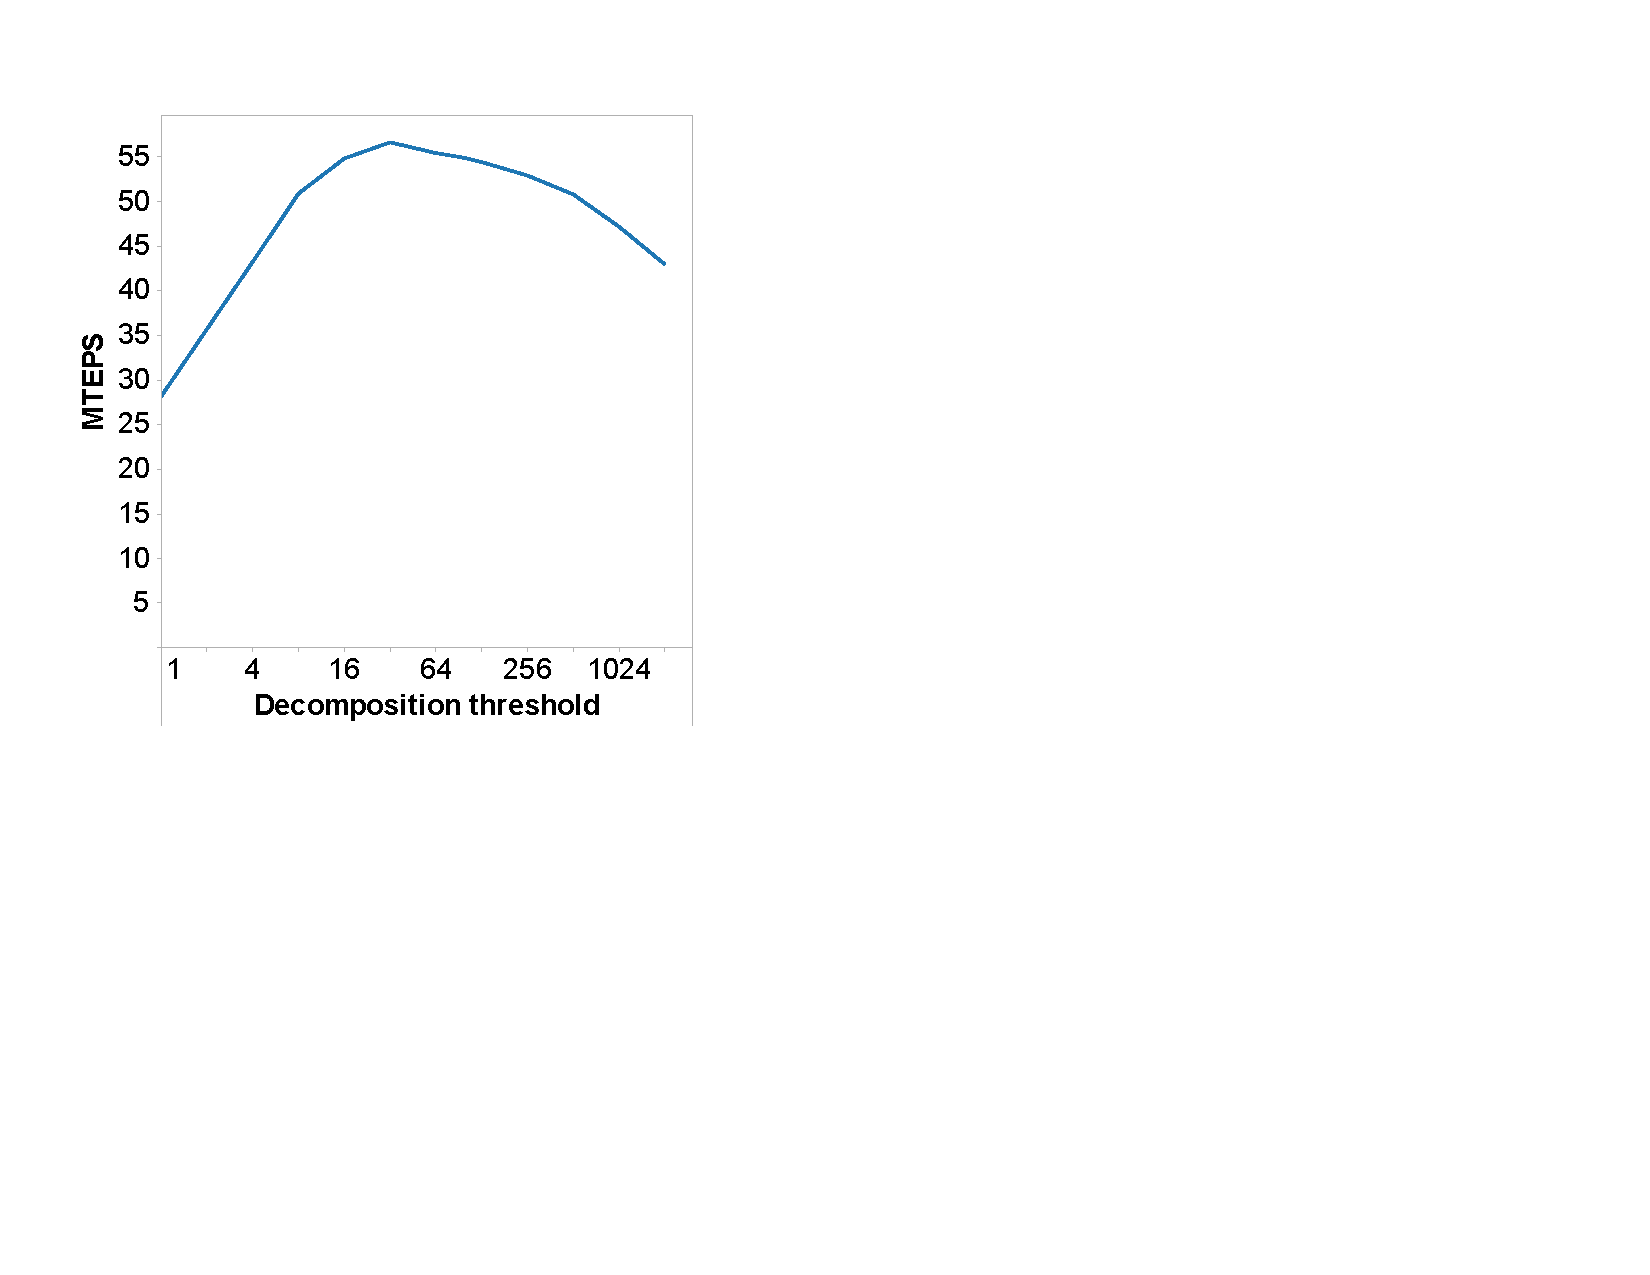
\includegraphics[width=0.95\columnwidth]{figs/bfs_sweep_threshold}
\begin{minipage}{0.95\columnwidth}
  \caption{\label{fig:bfs-sweep-threshold} Sensitivity to parallel loop threshold. Note the log scale.}
\end{minipage}
\vspace{-3ex}
\end{center}
\end{figure}

Parallel overhead---in the form of context switches, task spawns, and
synchronization---can reduce the performance benefit of parallelism.
Grappa sees a benefit to limiting the amount of parallelism created by
a recursive loop decomposition. The parallel loop threshold (``parallel
granularity'') parameter tells the runtime when to stop creating new tasks and just execute iterations
sequentially. This allows us to amoritize the overhead of task
creation. In addition, assigning sequential iterations to a single
task provides the potential to exploit locality when data for adjacent iterations is
also adjacent in memory.

Figure~\ref{fig:bfs-sweep-threshold} shows a sweep of this parameter
for a 32-node BFS run. We saw the best results serializing 32 or fewer
iterations.

% uts threshold
\begin{figure}[ht]
    \begin{center}
      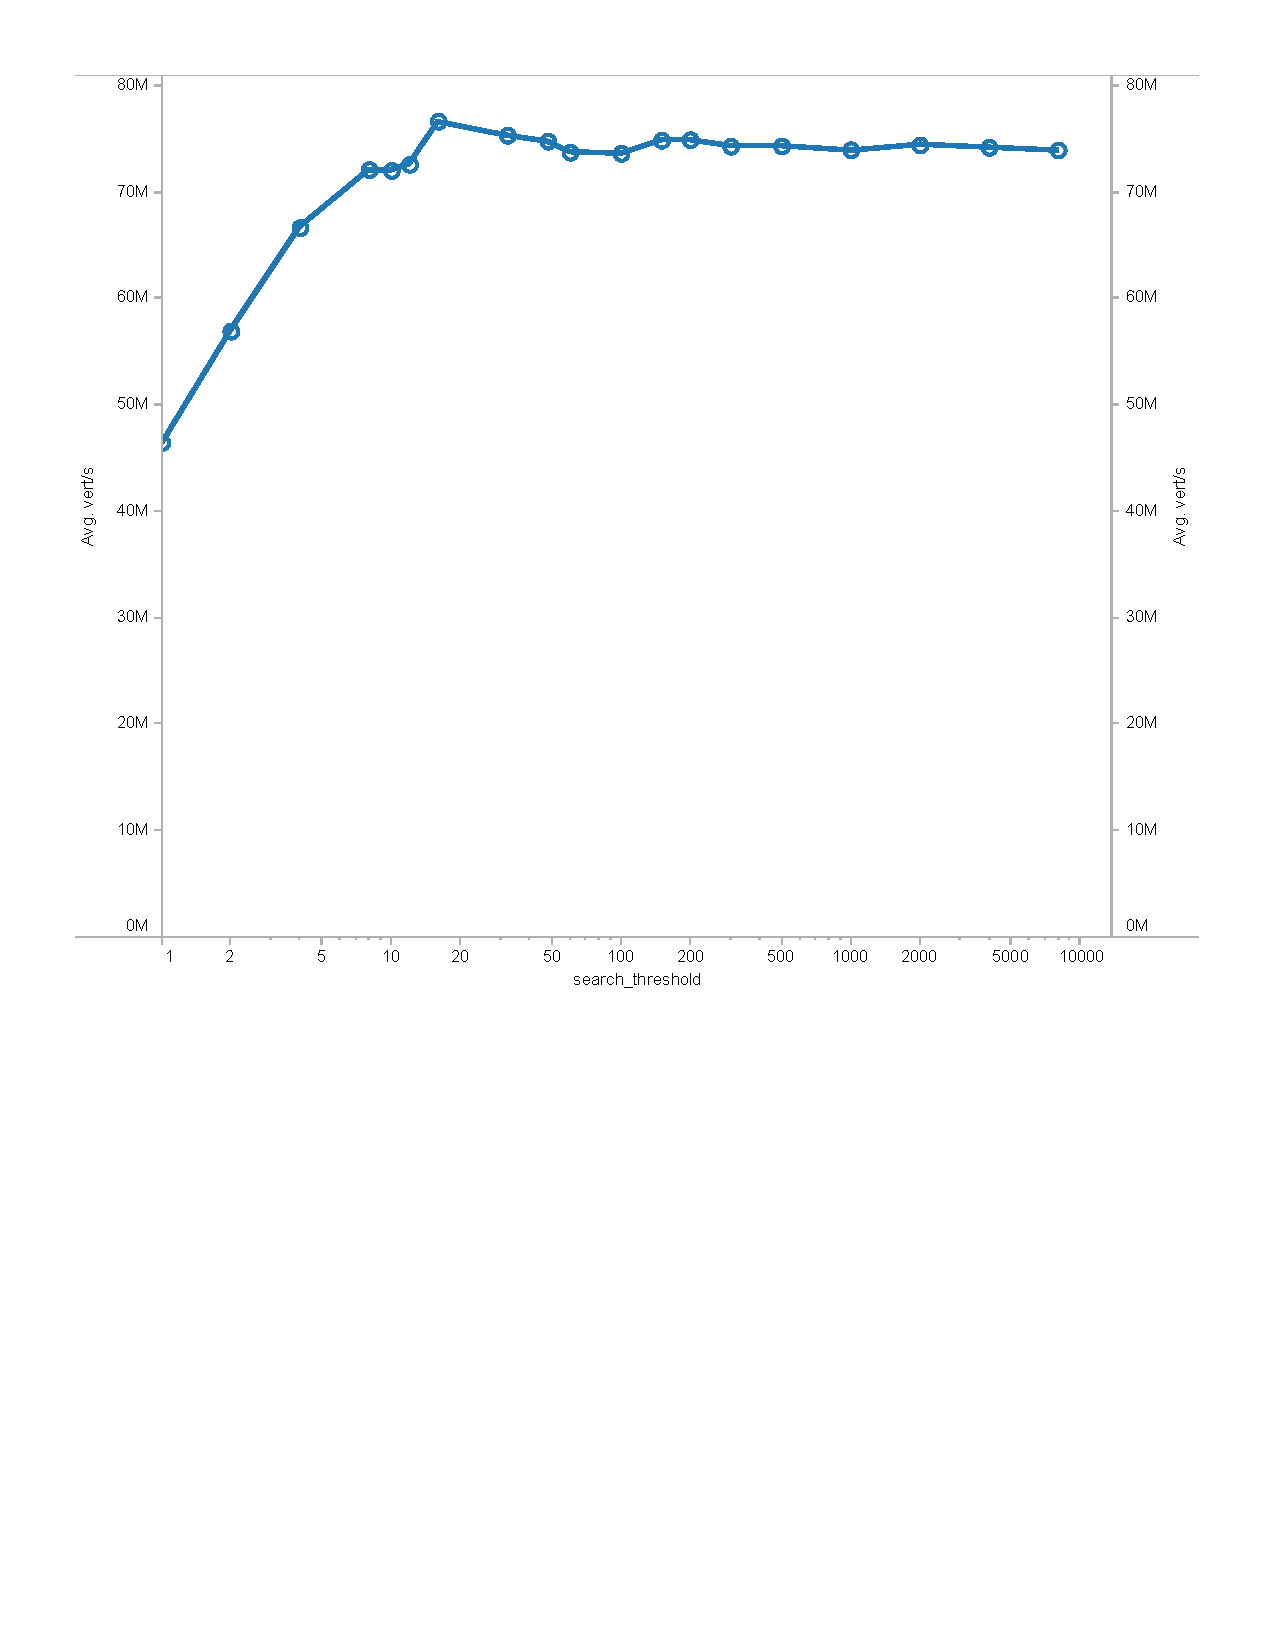
\includegraphics[width=0.5\textwidth]{figs/uts_threshold.pdf}
    \end{center}
    \caption{Performance of UTS-Mem with varying parallel loop
        threshold, run with 30 nodes, 6 cores per node, 4000 workers,
    \checkme{6M flush ticks}}
    \label{fig:uts_threshold}
\end{figure}

\subsection{Scaling}
\paragraph{UTS-Mem}
We ran UTS-Mem on Grappa and the XMT with a geometric 1.6B-vertex tree
(T1XL) and a geometric 4.2B-vertex tree (T1XXL), using up to 128
nodes---the maximum we had available for each. Grappa results are for 5 cores per node. Grappa with 20 machines is faster than the entire XMT of 128 processors.
Grappa achieves \checkme{188Mvert/s} with 128 nodes and the XMT
achieves only 50Mvert/s, plateauing at 60 nodes. Beyond 90 nodes, Grappa adds 1.4 Mvert/s/node.
The XMT scales at 850 Kvert/s/node, until it plateaus. Grappa keeps
scaling up through 128 nodes, although scaling
declines because of the unscalability of our aggregation mechanism as
number of network endpoints increases. 

Despite our efforts to tune the UTS implementation specific to the 
XMT, performance does not scale well with increasing processor count,
flattening out around 60 processors.  When we increase the size of
the tree from 100M to 4.2B, we find that performance does not improve,
suggesting that performance is not limited by task parallelism.
Cray's performance tools show an increasing number of memory
retry operations for failed synchronization operations generated by
the runtime, which create network contention.
%Retries are performed by the memory controller when remote synchronization operations fail to find the full-bit associated with each memory location in the unavailable state.  Retries are issued at low priority relative to new memory operations issued by the processor by other contexts, so they consume what would otherwise be unused injection bandwidth.  On a full-bandwidth system such as the MTA-2, retries have no impact on the progress of tasks other than their own.  On a Cray XMT, network bandwidth is limited, so retries create congestion.  In comparison, Grappa performs synchronization without retries, delaying responses at the receiving end until ready to notify the sender to proceed.  This saves bandwidth and permits scaling of tasks performing synchronization even on low injection rate networks.


%\begin{figure*}[ht]
%    \begin{minipage}{0.3\linewidth}
%        \centering
%        \includegraphics[width=\textwidth]{figs/chunksize-uts.pdf}
%        \caption{chunksize caption}
%        \label{fig:chunksize-uts}
%    \end{minipage}
%    \begin{minipage}{0.3\linewidth}
%        \centering
%        \includegraphics[width=\textwidth]{figs/workers-uts.pdf}
%        \caption{workers caption}
%        \label{fig:workers-uts}
%    \end{minipage}
%    \begin{minipage}{0.3\linewidth}
%        \centering
%        \includegraphics[width=\textwidth]{figs/thresh-uts.pdf}
%        \caption{threshold caption}
%        \label{fig:thresh-uts}
%    \end{minipage}
%\end{figure*}
